\section{Einschränkung der Bewegung in die Ebene}
Das der Drehimpuls zeitlich konstant ist, erlaubt es uns, die Bewegung auf die Betrachtung in der Ebene einzuschränken. Dazu nehmen wir an, dass für die $z$-Komponenten der Anfangswerte
\[
  \vec{x}_{0,3} = \dot{\vec{x}}_{0,3} = 0
\]
gilt, und das $\vec{x}$ und $\dot{\vec{x}}$ linear unabhängig sind.
Für die Komponenten des Drehimpulses gilt jetzt
\begin{align*}
\vec{L} = m(\vec{x}\times \dot{\vec{x}}) &= m\cdot \begin{pmatrix} x_1\\x_2\\x_3\end{pmatrix} \times \begin{pmatrix}
  \dot{x}_1,\\\dot{x}_2\\\dot{x}_3\end{pmatrix}\\
  &= \begin{pmatrix} x_2 \dot{x}_3-x_3\dot{x}_2\\ x_3\dot{x}_1 - x_1\dot{x}_3\\ x_1\dot{x}_2 - x_2\dot{x}_1\end{pmatrix}
\end{align*}
Da aber $\vec{L}=\mathrm{const.}$ gilt, ist
\[
\vec{L} =m \begin{pmatrix} 0\\0\\x_{0,1}\dot{x}_{0,2} - x_{0,2}  \dot{x}_{0,1}\end{pmatrix}
\]
Also steht der Drehimpulsvektor senkrecht auf der von $\vec{x}$ und $\dot{\vec{x}}$ aufgespannten Ebene. Wir definieren weiterhin
\[
L:= m(x_{0,1}\dot{x}_{0,2} - x_{0,2}  \dot{x}_{0,1}).
\]
Weiterhin gilt
\[
\langle \vec{L},\vec{x}\rangle = \langle \vec{L},\dot{\vec{x}} \rangle = 0,
\]
so dass sowohl $\vec{x}$ und $\dot{\vec{x}}$ die ganze Zeit senkrecht auf $\vec{L}$ stehen, also die Bewegung die ganze Zeit in der $x$-$y$-Ebene stattfindet. Diese Erkenntnis ist extrem wichtig, und stellt eine unglaublich nützliche Einschränkung der Bewegung dar. \par
Um sie vollständig ausnutzen zu können, werden wir nun eine Koordinatentransformation durchführen, und das System in \emph{Polarkoordinaten} beschreiben. Dazu schreiben wir
\[
\vec{x} = \begin{pmatrix} r\cos \theta\\ r\sin \theta \end{pmatrix},
\]
wobei
\[
r:= \sqrt{x_1^2+x_2^2}~\text{und}~\theta := \arctan\left(\frac{y}{x}\right).
\]
\begin{figure}[h]
  \centering
  \begin{tikzpicture}
    \tkzInit[xmax=1.2,ymax=1.2,ymin=-1.2,xmin=-1.2]
    \tkzGrid
    \tkzDefPoint(0,0){A}
    \tkzDefPoint(1,0){B}
    \tkzDrawCircle[R](A,1cm)
    \tkzDefPointBy[rotation in rad= center A angle pi/4](B)
    \tkzGetPoint{C}
    \tkzDrawPoints(A,B,C)
    \tkzDrawSegment(A,C)
    \tkzLabelSegment[above, pos =.5](A,C){$r$}
    \tkzMarkAngle[size = .3cm](B,A,C)
    \tkzLabelAngle[below left](B,A,C){$\theta$}
  \end{tikzpicture}
\end{figure}
In diesen Koordinaten gilt jetzt
\[
\dot{\vec{x}} = \begin{pmatrix} \dot{r} \cos\theta - r\dot{\theta}\sin\theta\\ \dot{r}\sin\theta + r\dot{\theta} \cos\theta\end{pmatrix}
\]
Setzen wir dies in die Definitionen von Drehimpuls und Energie ein, dann erhalten wir
\begin{align*}
L &= mr^2\dot{\theta}\\
E &= \frac{1}{2}m(\dot{r}^2+r^2\dot{\theta}^2)-\frac{k}{r}
\end{align*}
Aber wir können noch mehr machen. Weil wir wissen, dass $L$ konstant ist, stellen können wir die \emph{Winkelgeschwindigkeit} $\dot{\theta}$ durch $L$ und $r$ ausdrücken\footnote{$r$ wird nie null sein, weil aus unseren Annahmen $L\neq0$ für alle Zeiten folgt.}
\[
\dot{\theta} = \frac{L}{mr^2} \implies E = \frac{1}{2}m\dot{r}^2 + \underbrace{\frac{L^2}{2mr^2}- \frac{k}{r}}_{=: \phi_{eff}}
\]
Die Größe $\phi_{eff}$ nennen wir \emph{effektives Potential} der Bewegung.\\
Auf einmal haben wir es erreicht, dass wir die Energie durch nur noch eine Koordinate, und nicht mehr wie anfänglich drei Koordinaten, ausdrücken können. \par
Wir wollen das nun nutzen, um zu verstehen, welche Werte für $r$ jeweils möglich sind. Dazu nehmen wir für den Moment vereinfachend $k=m=1$ an, und betrachten die Funktion $1/r^2-1/r$: und die Fälle $E_1>0$, $E_2<0$ sowie $E_{2^\ast}=-1/4$.
\begin{figure}[h]
  \centering
  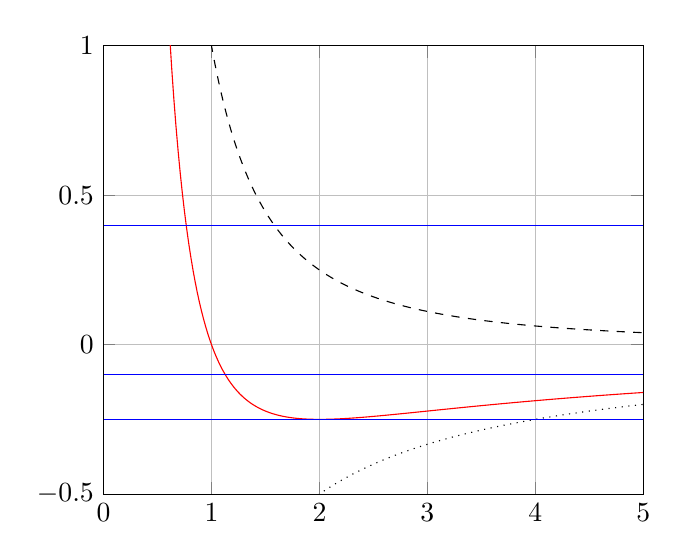
\begin{tikzpicture}
    \begin{axis}[xmin = 0,xmax = 5, ymin=-.5,ymax=1,grid = major
      ]
      \addplot[red,domain=0.1:5,samples=250]{1/x^2-1/x};
      \addplot[dashed,domain=0.1:5,samples =250]{1/x^2};
      \addplot[dotted,domain=0.1:5,samples =250]{-1/x};
      \addplot[blue, domain=0:5,sharp plot,update limits=false]
        coordinates {(0,.4) (5,.4)};
      \addplot[blue, domain=0:5,sharp plot,update limits=false]
        coordinates {(0,-.1) (5,-.1)};
      \addplot[blue, domain=0:5,sharp plot,update limits=false]
        coordinates {(0,-.25) (5,-.25)};
    \end{axis}
  \end{tikzpicture}
\end{figure}
\paragraph*{Fall $1$: $E\geq 0$ - Unbeschränkte Bewegung}
Wir bezeichnen den Radius, für den $E=\phi_{eff}$ gilt, mit $r_i$. Dann stellen wir fest, dass das System keinen Zustand mit $r<r_i$ annehmen kann. In diesem Fall würde nämlich $\phi_{eff}>E$ gelten, und damit $\dot{r}^2<0$ seien müssen, was aber nicht möglich ist. Allerdings kann $r$ beliebig groß werden, weil $\phi_{eff}(r)<\phi_{eff}(r_0)$ für alle $r>r_0$ ist. Die Bewegung muss in diesem Fall also nicht beschränkt sein.
\paragraph*{Fall $2$: $E <0$ - beschränkte Bewegung}
Es gilt
\[
\lim_{r\to \infty} \frac{1}{r^2} - \frac{1}{r} = 0,
\]
und $\phi_{eff}(1) =0$. Also muss $\phi_{eff}$ ein irgendwo ein Minimum annehmen. Man kann jetzt auch noch nachrrechnen, dass $\phi_{eff}$ auf $(0,1/2)$ streng monoton fallend ist, und auf $(1/2,\infty)$ streng monoton wachsend. Also gibt es für gegebenes $E\in (0,1/4)$ genau zwei Radii $r_a,r_b$ sodass $U_{eff}=E$ gilt. Nach der gleichen Argumentation wie im Fall 1 ist aber eine Bewegung mit $U_{eff}>E$ nicht möglich, so dass in diesem Fall die Bewegung durch Kreise mit den Radii $r_a,r_b$ beschränkt ist. Wir wissen aber zum Beispiel noch nicht, ob die Bahn geschlossen oder periodisch ist.
\paragraph*{Fall $2^\ast$: $E=U_{eff,min}$ - Kreisbahn}
Das lokale Minimum, und die zugehörige Extremalstelle $R$, von $\phi_{eff}$ erhalten wir, wie üblich, durch Ableiten nach $r$ und null-setzen:
\[
0\overset{!}{=}\phi'_{eff}(R) = -\frac{L^2}{mR^3}+\frac{k}{R} \implies R = \frac{L^2}{km}
\]
Findet die Bewegung bei dieser Energie statt, dann folgt aus der Überlegung für $E<0$ aber bereits, dass hier $r_a=r_b=R$ gelten muss. Also muss $r$ die ganze Zeit konstant $R$ sein, also ist die Bahn durch eine Kreisbahn gegeben.
